\chapter{Canonical Quantization}

    The main reference for this chapter is~\citet{peskin_introduction_1995}. For the section on the Connes--Kreimer algebra, see the original paper by~\citet{connes_hopf_1998}.

\section{Klein--Gordon field}\index{Klein--Gordon equation}
\subsection{Lagrangian and Hamiltonian}

    The `simplest' Lagrangian (density) is given by
    \begin{gather}
        \label{qft:klein_gordon_lagrangian}
        \mathcal{L} = \frac{1}{2}\partial_\mu\phi\partial^\mu\phi - \frac{1}{2}m^2\phi^2\,.
    \end{gather}
    Using the principle of least action, the following Euler--Lagrange equation is obtained:
    \begin{gather}
        \left(\partial^\mu\partial_\mu + m^2\right)\phi = 0\,.
    \end{gather}
    This can be rewritten using the \textbf{d'Alembertian} $\Box = \partial_\mu\partial^\mu$:\index{d'Alembert!operator}
    \begin{gather}
        \label{qft:klein_gordon_equation}
        (\Box+m^2)\phi = 0\,.
    \end{gather}
    This equation is called the \textbf{Klein--Gordon equation}. In the limit $m\longrightarrow0$, this equation reduces to the well-known wave equation (\cref{optics:wave_equation}).

    From the Lagrangian~\eqref{qft:klein_gordon_lagrangian}, one can also derive a Hamiltonian function using \cref{lagrange:conjugate_momentum} and \cref{lagrange:hamiltonian}:
    \begin{gather}
        \label{qft:klein_gordon_hamiltonian}
        H = \frac{1}{2}\Int_{\mathbb{R}^3}\left[\pi^2(x) + (\nabla\phi(x))^2 + m^2\phi^2(x)\right]\,d^3x\,.
    \end{gather}

\subsection{Raising and lowering operators}

    Fourier transforming the scalar field $\phi(\mathbf{x})$ and inserting it into the Klein--Gordon equation gives
    \begin{gather}
        \left(\partial_t^2+p^2+m^2\right)\phi(\mathbf{p}) = 0\,.
    \end{gather}
    This is the equation for a simple harmonic oscillator with frequency $\omega = \sqrt{p^2+m^2}$.

    Analogous to ordinary quantum mechanics, raising and lowering operators $a_{\vector{p}}^\dag$ and $a_{\vector{p}}$ can be defined such that
    \begin{align}
        \phi(\vector{x}) &= \Int_{\mathbb{R}^3}\frac{d^3p}{(2\pi)^{3/2}}\frac{1}{\sqrt{2\omega_{\vector{p}}}}\left(a_{\vector{p}}e^{i\vector{p}\cdot\vector{x}} + a_{\vector{p}}^\dag e^{-i\vector{p}\cdot\vector{x}}\right)\,,\label{qft:phi}\\
        \pi(\vector{x}) &= \Int_{\mathbb{R}^3}\frac{d^3p}{(2\pi)^{3/2}}(-i)\sqrt{\frac{\omega_{\vector{p}}}{2}}\left(a_{\vector{p}}e^{i\vector{p}\cdot\vector{x}} - a_{\vector{p}}^\dag e^{-i\vector{p}\cdot\vector{x}}\right)\,.
    \end{align}
    An equivalent definition is obtained by performing the transformation $\vector{p}\longrightarrow-\vector{p}$ in the second term of $\phi(\vector{x})$ and $\pi(\vector{x})$:
    \begin{align}
        \phi(\vector{x}) &= \Int_{\mathbb{R}^3}\frac{d^3p}{(2\pi)^{3/2}}\frac{1}{\sqrt{2\omega_{\vector{p}}}}\left(a_{\vector{p}} + a_{-\vector{p}}^\dag\right)e^{i\vector{p}\cdot\vector{x}}\,,\\
        \pi(\vector{x}) &= \Int_{\mathbb{R}^3}\frac{d^3p}{(2\pi)^{3/2}}(-i)\sqrt{\frac{\omega_{\vector{p}}}{2}}\left(a_{\vector{p}} - a_{-\vector{p}}^\dag\right)e^{i\vector{p}\cdot\vector{x}}\,.
    \end{align}

    When the commutation relation
    \begin{gather}
        \label{qft:ladder_comutation}
        [a_{\vector{p}},a_{\vector{q}}^\dag] := \delta(\vector{p}-\vector{q})
    \end{gather}
    is imposed, the following commutation relation for the scalar field and its conjugate momentum is obtained:
    \begin{gather}
        [\phi(\vector{x}),\pi(\vector{y})] = i\delta(\vector{x} - \vector{y})\,.
    \end{gather}
    Now, the Hamiltonian can be calculated explicitly:
    \begin{gather}
        \label{qft:Klein_gordon_hamiltonian}
        H = \Int_{\mathbb{R}^3}\frac{d^3p}{(2\pi)^3}\omega_{\vector{p}}\left(a_{\vector{p}}^\dag a_{\vector{p}} + \frac{1}{2}[a_{\vector{p}},a_{\vector{p}}^\dag]\right)\,.
    \end{gather}
    However, it is clear from \cref{qft:ladder_comutation} that the second term in this integral diverges. There are two reasons for this divergence. First, space is infinite, i.e.~the $d^3x$ integral in \cref{qft:klein_gordon_hamiltonian} diverges. This problem can be resolved by restricting the system to a (finite) part of space or by considering the energy density instead of the energy itself. Second, by including very large values for $p$ in the integral, a parameter range is explored where the theory is likely to break down. To resolve this problem a  `high $p$'-cut-off should be introduced. A more practical solution, however, is to note that only energy differences are physical and so one can simply drop the second term altogether as it is merely a `constant' (albeit an infinite one).

    A corollary of \cref{qft:Klein_gordon_hamiltonian} together with the canonical commutation relations is
    \begin{align}
        [H,a_{\vector{p}}^\dag] &= \omega_pa_{\vector{p}}^\dag\,,\\
        [H,a_{\vector{p}}] &= -\omega_pa_{\vector{p}}\,.
    \end{align}
    As was the case for the quantum harmonic oscillator, the creation and annihilation operators deserve their names and one can write:
    \begin{gather}
        |\vector{k}_1,\ldots,\vector{k}_n\rangle = a^\dag(\vector{k}_1)\cdots a^\dag(\vector{k}_n)|0\rangle\,.
    \end{gather}
    Furthermore, this equation together with the canonical commutation relations imply that the Klein--Gordon fields are bosonic fields. This way of generating the full Hilbert (or, in fact, Fock) state space is axiomatized by the GNS construction (\cref{operators:gns}), where the vacuum plays the role of cyclic vector.

\subsection{Scalar propagator}

    \newformula{Pauli--Jordan function}{\index{Pauli--Jordan function}
        \begin{gather}
            i\Delta(\mathbf{x}-\mathbf{y}) := i[\phi(\mathbf{x}),\phi(\mathbf{y})] = \Int_{\mathbb{R}^3}\frac{d^3p}{(2\pi)^3}\frac{1}{2\omega_{\mathbf{x}}}\left(e^{-i\mathbf{p}\cdot(\mathbf{x}-\mathbf{y})} - e^{i\mathbf{p}\cdot(\mathbf{x}-\mathbf{y})}\right)
        \end{gather}
        When $x^0=y^0$ (ETCR) or $(\mathbf{x}-\mathbf{y})^2 < 0$ (spacelike curves), the Pauli--Jordan function is identically 0. (See also the \textit{axiom of microcausality}~\ref{aqft:microcausality}).
    }

\subsection{Normalization constant}

    By \cref{distribution:delta_of_function}, the delta function $\delta^{(3)}(\vector{p}-\vector{q})$ transforms as $\delta^{(3)}(\Lambda\vector{p} - \Lambda\vector{q})\frac{\Lambda E}{E}$ under a general Lorentz boost $\Lambda$. Although this is clearly not Lorentz invariant, the quantity $E_{\mathbf{x}}\delta^{(3)}(\vector{p}-\vector{q})$ can be seen to be invariant. From this observation it follows, that the correct normalization in the momentum representation is
    \begin{gather}
        |\mathbf{p}\rangle = \sqrt{2E_{\mathbf{x}}}a_{\mathbf{p}}^\dag|0\rangle
    \end{gather}
    and, hence,
    \begin{gather}
        \langle\mathbf{p}\mid\mathbf{q}\rangle = 2E_{\mathbf{x}}(2\pi)^3\delta^{(3)}(\vector{p}-\vector{q})\,,
    \end{gather}
    where the constants are a matter of convention to cancel the constants in \cref{qft:phi}.

\subsection{Invariant integration measure}

    The factor $2E_p$ does not only occur in the normalization conditions. To find a Lorentz-invariant integration measure in spacetime, the following integral can be studied:
    \begin{gather}
        \Int_{\mathbb{R}^3}\frac{d^3p}{2E_p} = \Int_{\mathbb{R}^+\times\mathbb{R}^3}\delta(p^2-m^2)\,d^4p\,,
    \end{gather}
    where the timelike component $p^0$ is restricted to be (strictly) positive. By using this measure, it is ensured that the integral of any Lorentz-invariant function is again Lorentz invariant.
    \begin{example}[One-particle identity operator]\index{identity!operator}
        \begin{gather}
            \mathbbm{1} := \Int_{\mathbb{R}^3}\frac{d^3p}{2E_p}|\mathbf{p}\rangle\langle\mathbf{p}|
        \end{gather}
    \end{example}

\section{Contractions and Wick's theorem}
\subsection{Bosonic fields}

    In the following definitions, (field) operators will be decomposed as \[\phi = \phi^{(+)} + \phi^{(-)}\,,\] where the + symbol denotes the `positive-frequency' part, i.e.~the part consisting of annihilation operators. The `negative-frequency' part is defined analogously. This terminology stems from classic Fourier theory. By looking at \cref{qft:phi} and remembering that the $(1,3)$-signature is adopted, the annihilators can be seen to always occur together with a positive-frequency exponential.

    \newdef{Contraction for neutral bosonic fields}{\index{contraction}
        \begin{gather}
            \contraction{}{\phi}{(\mathbf{x})}{\phi}\phi(\mathbf{x})\phi(\mathbf{y}) :=
            \begin{cases}
                [\phi(\mathbf{x})^{(+)},\phi(\mathbf{y})^{(-)}]&\cif x^0>y^0\\
                [\phi(\mathbf{y})^{(+)},\phi(\mathbf{x})^{(-)}]&\cif y^0>x^0
            \end{cases}
        \end{gather}
    }
    \newformula{Feynman propagator}{\index{Feynman!propagator}\label{qft:feynman_propagator_contraction}
        \begin{gather}
            i\Delta_F(\mathbf{x}-\mathbf{y}) := \contraction{}{\phi}{(\mathbf{x})}{\phi}\phi(\mathbf{x})\phi(\mathbf{y}) := i\lim_{\varepsilon\rightarrow 0^+}\Int_{\mathbb{R}^4}\frac{d^4p}{(2\pi)^4}\frac{e^{-i\mathbf{p}\cdot(\mathbf{x}-\mathbf{y})}}{p^2 - m^2 + i\varepsilon}
        \end{gather}
    }

    \newdef{Contraction for charged bosonic fields}{
        \begin{gather}
            \contraction{}{\phi}{(\mathbf{x})}{\overline\phi}\phi(\mathbf{x})\overline\phi(\mathbf{y}) :=
            \begin{cases}
                [\phi(\mathbf{x})^{(+)},\overline\phi(\mathbf{y})^{(-)}]&\cif x^0>y^0\\
                [\phi(\mathbf{y})^{(+)},\overline\phi(\mathbf{x})^{(-)}]&\cif y^0>x^0
            \end{cases}
        \end{gather}
    }

    \newdef{Normal ordering}{\index{normal!ordering}
        The normal ordering $\mathcal{N}$, often denoted by colons $:\ \ :$, of a sequence of field operators is defined as the permuted sequence in which all annihilation operators appear on the right of the creation operators, e.g.:
        \begin{gather}
            \mathcal{N}\bigl(\phi(\mathbf{x})\phi^\dag(\mathbf{y})\phi(\mathbf{z})\bigr) = \phi^\dag(\mathbf{y})\phi(\mathbf{x})\phi(\mathbf{z})\,.
        \end{gather}
        Note that the normal ordering operator is not a morphism between CCR-algebras since this would lead to a contradiction:
        \begin{gather}
            b_ib_j^\dag = b_j^\dag b_i + \delta_{ij}\implies\mathcal{N}(b_ib_j^\dag) = \mathcal{N}(b_j^\dag b_i+\delta_{ij}) = \mathcal{N}(b_j^\dag b_i) + \delta_{ij}\implies\delta_{ij}=0\,.
        \end{gather}
        The solution is given by the fact that inside the normal ordering all operators commute and, hence, this ordering can be axiomatized as an algebra morphism $\mathcal{N}:\Sym^\bullet A\rightarrow A$, where $A$ is the CCR-algebra of the theory (see~\citet{miwa_solitons_2000}).

        \todo{IS THIS REFERENCE CORRECT?}
    }
    \begin{property}
        From this definition, it immediately follows that the vacuum expectation value of a normal ordered sequence is 0.
    \end{property}

    \newformula{Wick's theorem for bosonic fields}{\index{Wick}
        \begin{gather}
            \mathcal{T}\bigl(\phi(\mathbf{x}_1)\cdots\phi(\mathbf{x}_n)\bigr) = \mathcal{N}\bigl(\phi(\mathbf{x}_1)\cdots\phi(\mathbf{x}_n) + \text{all possible contractions}\bigr)
        \end{gather}
        When acting with a time-ordered product on the vacuum, this relation implies that only fully contracted terms will remain. Moreover, by \cref{qft:feynman_propagator_contraction}, every such action can be expressed solely in terms of propagators.
    }

    \begin{remark}
        In the case of charged bosons, only contractions of the form $\contraction{}{\phi}{(\mathbf{x})}{\overline\phi}\phi(\mathbf{x})\overline\phi(\mathbf{y})$ will remain because $[a,b^+]=0$.
    \end{remark}

    \begin{result}
        \begin{gather}
            \contraction{}{\phi}{(\mathbf{x})}{\phi}\phi(\mathbf{x})\phi(\mathbf{y}) = \mathcal{T}\bigl(\phi(\mathbf{x})\phi(\mathbf{y})\bigr) - \mathcal{N}\bigl(\phi(\mathbf{x})\phi(\mathbf{y})\bigr)
        \end{gather}
    \end{result}

    Wick's theorem has an analogue in probability theory.
    \begin{theorem}[Isserlis]\index{Isserlis}
        Let $X_1,\ldots,X_n$ be a set of random variables following a multinormal distribution with mean 0.
        \begin{gather}
            \expect{X_1\cdots X_n} = \sum_{\sigma\in P_{n,2}}\prod_{\{i,j\}\in\sigma}\expect{X_iX_j}\,,
        \end{gather}
        where $P_{n,2}$ denotes the set of binary partitions of $\{1,\ldots,n\}$. Because the mean of the distribution is zero, this expression is equal to
        \begin{gather}
            \expect{X_1\cdots X_n} = \sum_{\sigma\in P_{n,2}}\prod_{\{i,j\}\in\sigma}\mathrm{cov}\bigl[X_i,X_j\bigr]\,.
        \end{gather}
    \end{theorem}

\subsection{Fermionic fields}

    \newdef{Contraction}{
        \begin{gather}
            \contraction{}{\psi}{(\mathbf{x})}{\overline\psi}\psi(\mathbf{x})\overline\psi(\mathbf{y}) :=
            \begin{cases}
                \{\psi(\mathbf{x})^{(+)},\overline\psi(\mathbf{y})^{(-)}\}_+&\cif x^0>y^0\\
                -\{\psi(\mathbf{y})^{(+)},\overline\psi(\mathbf{x})^{(-)}\}_+&\cif y^0>x^0
            \end{cases}
        \end{gather}
    }
    \begin{remark}
        Only contractions of the form $\contraction{}{\psi}{(\mathbf{x})}{\overline\psi}\psi(\mathbf{x})\overline\psi(\mathbf{y})$ will remain because $\{a,b^\dag\}_+=0$.
    \end{remark}

    \newformula{Feynman propagator}{\index{Feynman!propagator}
        \begin{gather}
            i\Delta_F(\mathbf{x}-\mathbf{y}) := \contraction{}{\psi}{(\mathbf{x})}{\overline\psi}\psi(\mathbf{x})\overline\psi(\mathbf{y}) := i\lim_{\varepsilon\rightarrow 0^+}\Int_{\mathbb{R}^4}\frac{d^4\mathbf{p}}{(2\pi)^4}\frac{\slashed{\mathbf{p}} + m}{p^2 - m^2 + i\varepsilon}e^{-i\mathbf{p}\cdot(\mathbf{x}-\mathbf{y})}
        \end{gather}
    }

    \begin{remark}[Normal ordering]
        One should take into account the Fermi--Dirac statistics when permuting fermionic field operators under a normal ordering. A general factor $\sgn(\sigma)$, where $\sigma$ is the permutation of the operators, will arise in every term, e.g.:
        \begin{gather}
            \mathcal{N}\bigl(\psi(\mathbf{x})\overline\psi(\mathbf{y})\psi(\mathbf{z})\bigr) = -\overline\psi(\mathbf{y})\psi(\mathbf{x})\psi(\mathbf{z})\,.
        \end{gather}
        A similar remark should be made for the time-ordering operator $\mathcal{T}$. As was the case for bosonic theories, one should pay attention to the nature of the normal ordering. It is not a morphism between CAR-algebras, but instead it is an algebra morphism between a free (odd) algebra and a CAR-algebra.
    \end{remark}

\section{Feynman rules}
\subsection{Scalar theory}

    By expanding the correlation functions in perturbation theory and applying Wick's theorem, one can rewrite every term using the following dictionary for Feynman diagrams (it is assumed that every coupling constant in the Lagrangian is divided by the necessary permutation factors, e.g.~in $\phi^4$-theory it is assumed that the constant is of the form $\lambda/4!$):
    \begin{itemize}
        \item Propagator $\Delta_F(\mathbf{x}-\mathbf{y})$:
            \begin{gather*}
                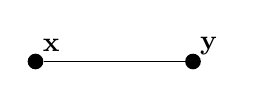
\begin{tikzpicture}
                    \node (labx) at (0.2,0.2) {$\mathbf{x}$};
                    \node (laby) at (2.2,0.2) {$\mathbf{y}$};
                    \node (x) at (0,0) [circle,fill,inner sep=2pt] {};
                    \node (y) at (2,0) [circle,fill,inner sep=2pt] {};
                    \draw (x) -- (y);
                \end{tikzpicture}
            \end{gather*}
        \item Interaction vertex\footnote{Four legs were drawn as an example but this can be generalized to any order of interaction term.} $-i\lambda\int d^4z$:
            \begin{gather*}
                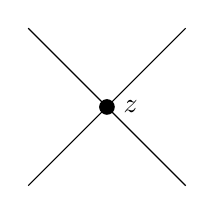
\begin{tikzpicture}
                    \node (z) at (0.3,0) {$z$};
                    \node (x) at (0,0) [circle,fill,inner sep=2pt] {};
                    \draw (-1,-1) -- (1,1);
                    \draw (-1,1) -- (1,-1);
                \end{tikzpicture}
            \end{gather*}
    \end{itemize}
    The main idea behind these rules is to draw all possible diagrams consistent with the given interaction Lagrangian and translate them into analytic expressions. However, to obtain the correct normalization, one should take the following remark into account.
    \begin{remark}\index{symmetry!factor}
        Symmetry factors of diagrams should be accounted for in analytic expressions. As an example, consider the following vacuum bubble:
        \begin{gather*}
            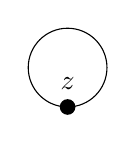
\begin{tikzpicture}
                \node (z) at (0, 0.3) {$z$};
                \node (x) at (0,0) [circle,fill,inner sep=2pt] {};
                \draw (0,0.5) circle (0.5);
            \end{tikzpicture}
        \end{gather*}
        Because the two legs can be interchanged, this diagram has \textbf{symmetry factor} 2 and, hence, it gives the analytic expression $-\frac{i\lambda}{2}\int d^4z\,\Delta_F(\mathbf{z}-\mathbf{z})$.
    \end{remark}

\section{Renormalization}

    One of the biggest issues in (quantum) field theory are the divergences that arise everywhere in calculations involving loop diagrams. Renormalization theory tries to find a way around these (nonphysical) divergences.

\subsection{Introduction: Statistical physics}

    Before introducing renormalization theory in the context of quatum field theory, it is helpful to study some applications in statistical physics, in particular in the study of lattice systems. To this end, this section will be focused on the study of the Ising model \ref{statmech:ising} on a lattice $\Lambda$:
    \begin{gather}
        \widehat{H} := -\sum_{\langle i,j \rangle\in\Lambda}J_{ij}\widehat{S}_i\widehat{S}_j-h\sum_{i\in\Lambda}\widehat{S}_i\,.
    \end{gather}

\subsection{Dimensional regularization}

    When calculating transition amplitudes and scattering cross-sections, three situations can arise:\index{divergence}
    \begin{enumerate}
        \item Convergence: Only low-energy/low-momentum contributions matter.
        \item UV divergence: These are sensivity to high-energy/high-momentum contributions, but only to these. Given a momentum cut-off, the integrals are fine.
        \item Logarithmic divergence: These get contributions from both low- and high-energy scales and, hence, a cut-off does not solve the issue.
    \end{enumerate}

    Consider the one-dimensional integral\footnote{Any integrand $g(x)\sim O(\frac{1}{x})$ will do.}
    \begin{gather}
        f_1(\theta) := \Int_0^{+\infty}\frac{1}{x+\theta}\,dx\,.
    \end{gather}
    For nonzero $\theta$, this integral has no IR divergence, but the upper bound still leads to trouble since $\ln(x)\xrightarrow{x\longrightarrow\infty}+\infty$. To this end, one can (formally) analytically continue the integral into a space `$\mathbb{R}^{1-\varepsilon}$'. This leads to the following regularization scheme:
    \begin{gather}
        f_{1,\varepsilon}(\theta) := \Int_0^{+\infty}\frac{x^{-\varepsilon}}{x+\theta}\,dx\,.
    \end{gather}
    Looking at \cref{calculus:beta_function}, this integral can be seen to be
    \begin{gather}
        f_{1,\varepsilon}(\theta) = \frac{B(\varepsilon,1-\varepsilon)}{\theta^\varepsilon}\,.
    \end{gather}
    Although this formula is finite for all $\theta\in\mathbb{R}$, it is now a function of $\varepsilon$ and actually diverges for $\varepsilon\longrightarrow0$ (which recovers the initial divergence).

    This is where renormalization comes in, where counterms are subtracted to remove the dependence on $\varepsilon$ and return a physical value. Here, the \textit{on-shell renormalization scheme} is adopted:\index{renormalization!on-shell}
    \begin{gather}
        f_1^R(\theta) := \lim_{\varepsilon\rightarrow0}\bigl(f_{1,\varepsilon}(\theta)-f_{1,\varepsilon}(1)\bigr) = \lim_{\varepsilon\rightarrow0}B(\varepsilon,1-\varepsilon)(\theta^{-\varepsilon}-1)\,.
    \end{gather}
    \cref{calculus:euler_reflection}, together with a Taylor expansion around $x=0$, show that this is finite for $\varepsilon\longrightarrow0$. If this were all, one could simply add counterterms for all such integrals. However, one also encounters interated integrals, corresponding to higher-order diagrams, and these should be regularized and renormalized as well. For a double integral, dimensional regularization gives:
    \begin{gather}
        f_{2,\varepsilon}(\theta) := \Int_0^{+\infty}\Int_0^{+\infty}\frac{x_1^{-\varepsilon}}{x_1+\theta}\frac{x_2^{-\varepsilon}}{x_2+x_1}\,dx_2\,dx_1 = \Int_0^{+\infty}\frac{x_1^{-\varepsilon}}{x_1+\theta}f_{1,\varepsilon}(x_1)\,dx_1\,.
    \end{gather}
    Naively subtracting a counterterm as for $f_1$, will, however, not work in this case since there are two (logarithmic) divergences. One for fixed $x_1$, when $x_2\longrightarrow+\infty$ and one when both $x_1,x_2\longrightarrow+\infty$. The former is called a \textbf{subdivergence}.\index{subdivergence}

    \begin{remark}[Nonlocality]
        The naive subtraction scheme $f_{2,\varepsilon}^R(\theta) := f_{2,\varepsilon}(\theta) - f_{2,\varepsilon}(1)$ can be found to be proportional to $\ln(\theta)$. In practice, the scale parameter $\theta$ is often related to the external momentum $q^2$. A term $\ln(q^2)$, however, points towards nonlocal behaviour since this term involves arbitrary high powers in $q^2$ or, after Fourier transforming back to position space, arbitrary high powers of a differential operator.
    \end{remark}

    First, one has to remove subdivergences. For $f_2$, this goes as follows:
    \begin{gather}
        \overline{f}_{2,\varepsilon}(\theta) := f_{2,\varepsilon}(\theta) - f_{1,\varepsilon}(\theta)f_{1,\varepsilon}(1)\,.
    \end{gather}
    A term consisting of the original function with the subdivergent factor set to 1, times that same contribution evaluated at $\theta=1$ is subtracted. In the next section, it will be shown how this procedure is generalized to arbitrary (logarithmically) divergent integrals. In the next step, one applies the `naive' subtraction scheme as for $f_1$:
    \begin{gather}
        f_2^R(\theta) := \lim_{\varepsilon\rightarrow0}\bigl(\overline{f}_{2,\varepsilon}(\theta)-\overline{f}_{2,\varepsilon}(1)\bigr)\,.
    \end{gather}

    To keep track of subdivergences, a diagrammatic method can be adopted. General integrals can be represented by rooted trees. Some examples are shown in \cref{fig:rooted_tree_subdivergences}. These trees correspond to the following divergent integrals:
    \begin{itemize}
        \item $f_{t_1}$:
        \begin{gather}
            \Int_0^{+\infty}\frac{x^{-\varepsilon}}{x+\theta}\,dx\,.
        \end{gather}
        \item $f_{t_2}$:
        \begin{gather}
            \Int_0^{+\infty}\frac{x_1^{-\varepsilon}f_{t_1}(x_1)}{x_1+\theta}\,dx_1\,.
        \end{gather}
        \item $f_{t_{3,1}}$:
        \begin{gather}
            \Int_0^{+\infty}\frac{x_1^{-\varepsilon}f_{t_2}(x_1)}{x_1+\theta}\,dx_1\,.
        \end{gather}
        \item $f_{t_{3,2}}$:
        \begin{gather}
            \Int_0^{+\infty}\frac{x_1^{-\varepsilon}f_{t_1}(x_1)f_{t_1}(x_1)}{x_1+\theta}\,dx_1\,.
        \end{gather}
    \end{itemize}

    \begin{figure}[t!]
        \centering
        \begin{tikzpicture}
            \begin{pgfonlayer}{nodelayer}
                \node [style=Circle, fill = black] (0) at (0, 1) {};
                \node [style=Circle] (1) at (0, -1) {};
                \node [style=Circle] (2) at (0, -3) {};
                \node [style=Circle, fill = black] (3) at (-2, 0) {};
                \node [style=Circle] (4) at (-2, -2) {};
                \node [style=Circle, fill = black] (5) at (-4, -1) {};
                \node [style=Circle, fill = black] (6) at (3, 0) {};
                \node [style=Circle] (7) at (2, -2) {};
                \node [style=Circle] (8) at (4, -2) {};
                \node [style=none] (9) at (-4, 2.5) {$t_1$};
                \node [style=none] (10) at (-2, 2.5) {$t_2$};
                \node [style=none] (11) at (0, 2.5) {$t_{3,1}$};
                \node [style=none] (12) at (3, 2.5) {$t_{3,2}$};
            \end{pgfonlayer}
            \begin{pgfonlayer}{edgelayer}
                \draw (3) to (4);
                \draw (0) to (2);
                \draw (7) to (6);
                \draw (6) to (8);
            \end{pgfonlayer}
        \end{tikzpicture}
        \caption{First four rooted trees.}
        \label{fig:rooted_trees_subdivergences}
    \end{figure}


\subsection{Wilsonian renormalization}

    \todo{COMPLETE}

 \subsection{Connes--Kreimer renormalization}\index{Connes--Kreimer renormalization}\index{grafting}\index{forest}

    The trees by which divergences and subdivergences in Feynman diagrams can be organized, admit an interesting algebraic structure. Consider the free commutative algebra $\mathcal{H}_R$ on rooted trees, where multiplication corresponds to juxtaposition (creating a `forest') with the empty tree as unit.

    $\mathcal{H}_R$ admits more structure then simply the addition and multiplication. It will be equipped with a Hopf algebra structure (\cref{nca:hopf_algebra}). The operations are defined as follows:
    \begin{itemize}
        \item Counit:
        \begin{gather}
            \varepsilon(\mathbf{1}):=1 \qquad\qquad\qquad \varepsilon(T):=0\,.
        \end{gather}
        \item Coproduct:
        \begin{gather}
            \Delta(T) := T\otimes\mathbf{1}+\mathbf{1}\otimes T+\sum_cP_c(T)\otimes R_c(T)\,,
        \end{gather}
        where the last term is a sum over all possible combinations of cuts for which any path from a vertex to the root only passes through at most one cut, i.e.~the \textbf{admissible cuts}.\footnote{Although, in theory, the two trivial cuts, where either $R_c(T)=\emptyset$ or $R_c(T)=T$, are also admissible, these are not included.} Given a cut $c$, the \textbf{trunk} $R_c(T)$ is the part of the tree that was attached to the root and the \textbf{branches} $P_c(T)$ is the forest given by all remaining components (this forest will consist of more than one tree if and only if $c$ contained multiples cuts).\index{trunk}\index{branch}
        \item Antipode (defined recursively):
        \begin{gather}
            S(\mathbf{1}) := \mathbf{1} \qquad\qquad\qquad S(T) := -T-\sum_cS\bigl(P_c(T)\bigr)R_c(T)\,.
        \end{gather}
    \end{itemize}
    Now, consider the operator $B_-:\mathcal{H}_R\rightarrow\mathcal{H}_R$ that removes the root from a tree (resulting in a forest) and the operator $B_+:\mathcal{H}_R\rightarrow\mathcal{H}_R$ that takes a forest of trees and grafts all of them to a new root. These can easily seen to be inverses. With these operators, the coproduct can be rewritten as follows:
    \begin{gather}
        \Delta(T) = T\otimes\mathbf{1} + (\mathbb{1}\otimes B_+)\circ\Delta\circ B_+(T)\,.
    \end{gather}

    The recursive expression for the antipode is the equation that ties in the Connes--Kreimer algebra with the substraction of subdivergent integrals from the previous section. The renormalized integrals are obtained through the antipode as follows:
    \begin{gather}
        f_T^R(\theta) := \lim_{\varepsilon\rightarrow0}\bigl([f_{S(T)}(\theta)] - f_{S(T)}(\theta)\bigr)\,,
    \end{gather}
    where the antipode on functions also incorporates the `bracket':
    \begin{gather}
        f_{S(T)} := -f_T - \sum_c\bigl[f_{S\left(P_c(T)\right)}\bigr]f_{R_c(T)}\,.
    \end{gather}
    The `bracket' corresponds to the choice of renormalization scheme, e.g.:
    \begin{itemize}
        \item On-shell renormalization:\index{renormalization!on-shell}
        \begin{gather}
            [f(\theta)] := f(1)\,.
        \end{gather}
        \item BPHZ\footnote{\textit{Bogoliubov, Parasiuk, Hepp} and \textit{Zimmermann}} renormalization:\index{renormalization!BPHZ}
        \begin{gather}
            [f(\theta)] := \mathrm{PolePart}_\varepsilon[f(1)]\,.
        \end{gather}
    \end{itemize}

    \todo{COMPLETE}

\section{Quantum chromodynamics}

	\newprop{OZI rule\footnotemark}{\index{OZI rule}
		\footnotetext{\textit{Okubo, Zweig} and \textit{Iizuka}}
        \nomenclature[A_OZI]{OZI}{Okubo--Zweig--Iizuka}
		Decay processes for which the corresponding Feynman diagrams become disconnected (initial states and final states are disconnected) when removing internal gluon lines, are suppressed with respect to other processes.
	}

\section{Entanglement in QFT}

    The main references are~\citet{tuybens_entanglement_2017,rangamani_holographic_2017}. This section should be seen as a generalization of \cref{chapter:quantum_computing} to the continuum setting, in particular the characterization and computation of entanglement.

\subsection{Lattice theories}

    In this section the most important definitions and constructions in ordinary quantum information theory are recalled and applied to a lattice theory. Taking the lattice spacing to zero will (formally) allow to extend the definitions to continuum field theories (up to some technicalities that will be explained when necessary). For simplicity, it will be assumed that the local Hilbert space is finite-dimensional.

    Consider a bipartite subdivision $A\cup A^c$ of the lattice, given by a codimension-1 hypersurface $\partial A$ called the \textbf{entangling surface}.\index{entangling surface} This induces a binary factorization of the total Hilbert space (all degrees of freedom are assumed to be confined to individual vertices) and, hence, one can compute the reduced density matrix for both $A$ and its complement $A^c$. The eigenvalues, which solely depend on the entangling surface $\partial A$, allow to calculate the von Neumann entropy:\footnote{Certain assumption ought to be made as to keep the entropy finite whenever the state-space is infinite-dimensional since it can be shown that the set of states with infinite von Neumann entropy is trace norm-dense (see~\citet{eisert_quantification_2002}).}
    \begin{gather}
        S(\rho_A) := -\tr(\rho_A\ln\rho_A) = -\sum_i\rho_i\ln\rho_i\,.
    \end{gather}
    In the same way one can also introduce the R\'enyi $q$-entropy:\index{entropy!R\'enyi}
    \begin{gather}
        S_q(\rho_A) := \frac{1}{1-q}\ln\Bigl(\sum_i\rho_i^q\Bigr)\,.
    \end{gather}
    \begin{property}[Limiting case]
         First of all one can analytically continue the definition of the $q$-entropy to arbitrary positive real numbers. The limit $q\longrightarrow1$ coincides with the von Neumann entropy.
    \end{property}

    @@ COMPLETE @@